
\section{Случайные блуждания на конечном множестве с отражающими экранами как марковская цепь}

\textbf{Автор:} Хайдари Фарид Гулович, Б-01-008

\subsection{Введение}
В данной работе рассматривается представление случайных блужданий на конечном множестве с отражающими экранами в виде марковской цепи. Здесь приводятся свойства данной марковской цепи, такие как периодичность, эргодичность и стационарность, и объясняется, как они связаны с характеристиками случайных блужданий. Также рассматриваются примеры применения марковских цепей в различных областях, таких как физика, экономика и биология, и объясняется, как случайные блуждания могут быть использованы для моделирования различных процессов.

\subsection{О марковских цепях}

\paragraph{Определение}

Одно из свойств, сильно упрощающее исследование случайного процесса — это «марковское свойство». Если объяснять очень неформальным языком, то марковское свойство сообщает нам, что если мы знаем значение, полученное каким-то случайным процессом в заданный момент времени, то не получим никакой дополнительной информации о будущем поведении процесса, собирая другие сведения о его прошлом. Более математическим языком: в любой момент времени условное распределение будущих состояний процесса с заданными текущим и прошлыми состояниями зависит только от текущего состояния, но не от прошлых состояний (\textbf{свойство отсутствия памяти}). Случайный процесс с марковским свойством называется \textbf{марковским процессом}.

$$
\mathbb{P}(\text{будущее} \  | \  \text{настоящее, прошлое}) = \mathbb{P}(\text{будущее} \  | \  \text{настоящее})
$$

Марковское свойство обозначает, что если мы знаем текущее состояние в заданный момент времени, то нам не нужна никакая дополнительная информация о будущем, собираемая из прошлого.

На основании этого определения мы можем сформулировать определение <<однородных цепей Маркова с дискретным временем>> (в дальнейшем для простоты мы их будем называть <<цепями Маркова>>). \textbf{Цепь Маркова} — это марковский процесс с дискретным временем и дискретным пространством состояний. Итак, цепь Маркова — это дискретная последовательность состояний, каждое из которых берётся из дискретного пространства состояний (конечного или бесконечного), удовлетворяющее марковскому свойству.

Рассмотрим цепь Маркова с конечным числом состояний $X = \{1, 2, ..., N\}$. Вероятности
\[
p_{ij}^{(n)} = \mathbb{P} (\xi_{m + n} = j | \xi_m = i), \  n \geq 1, \  m \geq 1, \  i, j \in X
\]
называются вероятностями перехода цепи Маркова за n шагов, а $p_{ij}$ = $p_{ij}$ просто вероятностями перехода. Матрица вида
\[
P = \begin{pmatrix}
p_{11} & p_{12} & \dots & p_{1N}\\
p_{21} & p_{22} & \dots & p_{2N}\\
\vdots & \vdots & \ddots & \vdots\\
p_{N1} & p_{N2} & \dots & p_{NN}
\end{pmatrix}
\]
называется матрицей вероятностей перехода цепи Маркова.

\paragraph{Свойства}

В данном разделе доклада мы рассмотрим свойства марковских цепей, в частности, свойства разложимости, апериодичности и возвратности. Неразложимость цепи Маркова означает, что из любого состояния можно достичь любого другого состояния с ненулевой вероятностью. Апериодичное состояние имеет период $d$, если для возврата в это состояние нужно количество этапов времени, кратное $d$, и является апериодическим, если апериодичны все её состояния. Невозвратное состояние имеет ненулевую вероятность того, что мы никогда в него не вернёмся, а возвратное состояние означает, что мы можем вернуться в него с вероятностью 1. Для возвратных состояний можно вычислить ожидаемое время возврата, которое может быть как конечным, так и бесконечным. В следующих разделах мы рассмотрим некоторые теоремы, связанные с марковскими цепями, и применения марковских цепей в различных областях.

\paragraph{Разложимость}

\textbf{Несущественным состоянием} $i \in X$ называется состояние, из которого можно за положительное число шагов выйти: $\exists m, j : p_{ij} > 0$, но нельзя в него вернуться: $\forall n : p_{ij} = 0$.

Если из множества $X$ всех состояний выделить несущественные, то оставшееся множество \textbf{существенных} состояний обладает тем свойством, что, попав в него, цепь Маркова никогда из него не выйдет.

\textbf{Сообщающимися состояниями} $i$ и $j$ называются существенные состояния, если $i$ достижимо из $j$, и $j$ достижимо из $i$ с ненулевой вероятностью. Обозначается как $i \leftrightarrow j$.

Множество существенных состояний разбивается на конечное или счетное число непересекающихся множеств $X_1 , X_2 , ...$ состоящих из сообщающихся состояний и характеризующихся тем, что переходы между различными множествами невозможны. Тогда такие множества называют \textbf{классами} или \textbf{неразложимыми классами} существенных сообщающихся состояний.

Цепь Маркова \textbf{неразложима}, если можно достичь любого состояния из любого другого состояния с ненулевой вероятностью (необязательно, что за один шаг времени). Если пространство состояний конечно и цепь можно представить в виде графа, то мы можем сказать, что граф неразложимой цепи Маркова сильно связный.
\begin{figure}[H]
    \centering
    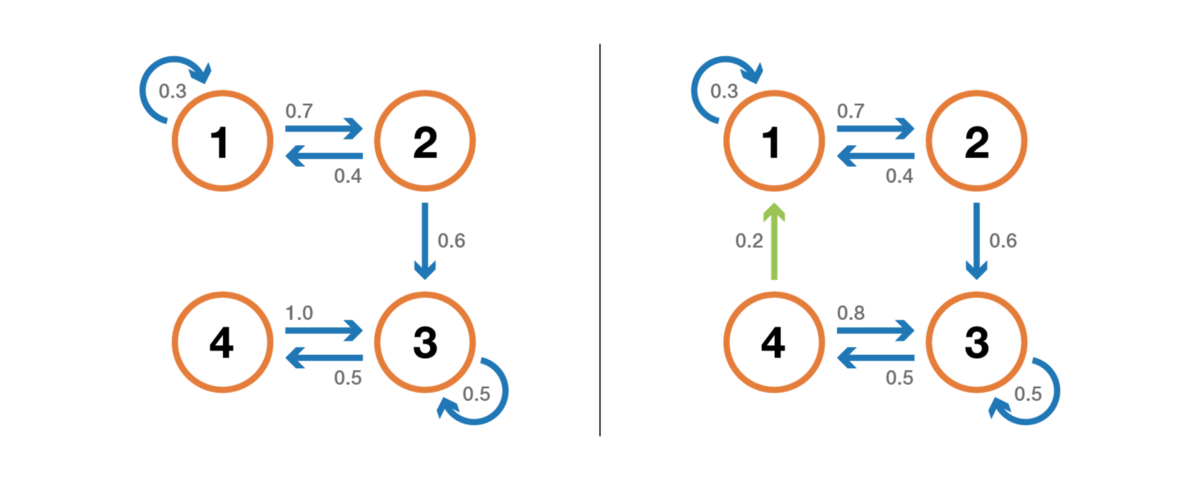
\includegraphics[width=0.6\textwidth]{fscanf_pic_razloshimost.png}
    \caption{Иллюстрация свойства неразложимости (несокращаемости). Цепь слева нельзя сократить: из $3$ или $4$ мы не можем попасть в $1$ или $2$. Цепь справа (добавлено одно ребро) можно сократить: каждого состояния можно достичь из любого другого с ненулевой вероятностью.}
\end{figure}

\paragraph{Апериодичность}

Состояние имеет период $d$, если при уходе из него для любого возврата в это состояние нужно количество этапов времени, кратное $d$ ($d$ -- наибольший общий делитель всех возможных длин путей возврата). Если $d = 1$, то говорят, что состояние является апериодическим, а вся цепь Маркова является \textbf{апериодической}, если апериодичны все её состояния. В случае неприводимой цепи Маркова можно также упомянуть, что если одно состояние апериодическое, то и все другие тоже являются апериодическими.
\begin{figure}[H]
    \centering
    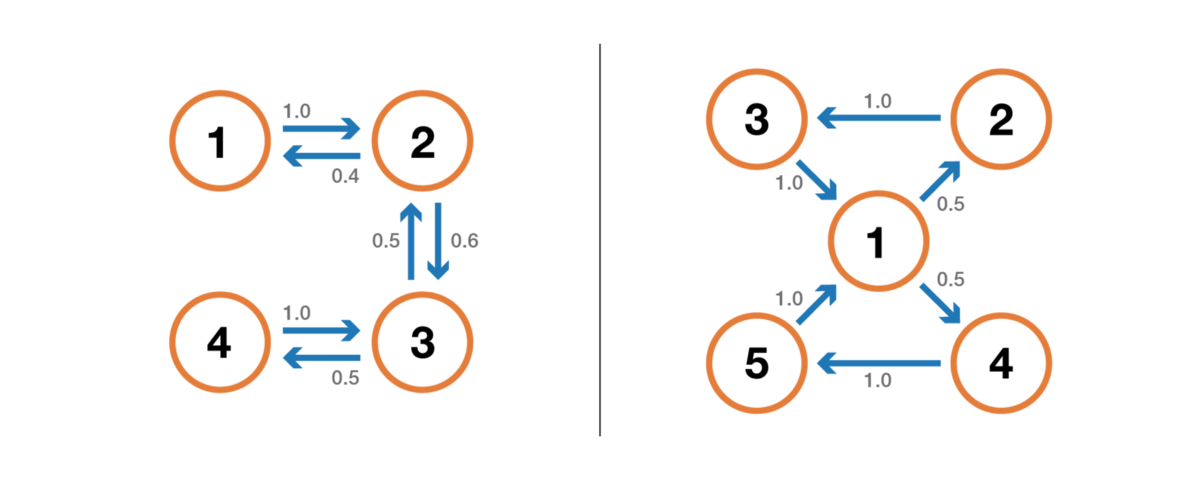
\includegraphics[width=0.6\textwidth]{fscanf_pic_aperiodichnost.png}
    \caption{Иллюстрация свойства периодичности. Цепь слева периодична с $d = 2$: при уходе из любого состояния для возврата в него всегда требуется количество шагов, кратное $2$. Цепь справа имеет период $3$}
\end{figure}

\paragraph{Возвратность}
Состояние является \textbf{невозвратным}, если при уходе из состояния существует ненулевая вероятность того, что мы никогда в него не вернёмся. И наоборот, состояние считается \textbf{возвратным}, если мы знаем, что после ухода из состояния можем в будущем вернуться в него с вероятностью 1 (если оно не является невозвратным).
\begin{figure}[H]
    \centering
    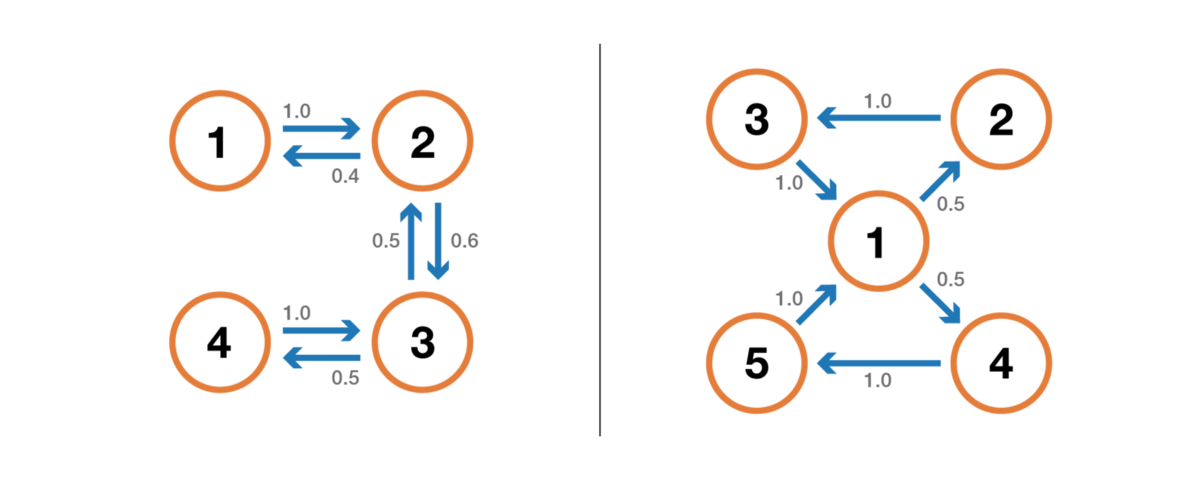
\includegraphics[width=0.6\textwidth]{fscanf_pic_aperiodichnost.png}
    \caption{Иллюстрация свойства возвратности/невозвратности. Цепь слева имеет такие свойства: $1$, $2$ и $3$ невозвратны (при уходе из этих точек мы не можем быть абсолютно уверены, что вернёмся в них) и имеют период $3$, а $4$ и $5$ возвратны (при уходе из этих точек мы абсолютно уверены, что когда-нибудь к ним вернёмся) и имеют период $2$. Цепь справа имеет ещё одно ребро, делающее всю цепь возвратной и апериодической.}
\end{figure}

Для возвратного состояния мы можем вычислить среднее время возвратности, которое является \textbf{ожидаемым временем возврата} при покидании состояния. Заметьте, что даже вероятность возврата равна $1$, то это не значит, что ожидаемое время возврата конечно. Поэтому среди всех возвратных состояний мы можем различать \textbf{положительные возвратные состояния} (с конечным ожидаемым временем возврата) и \textbf{нулевые возвратные состояния} (с бесконечным ожидаемым временем возврата).

\paragraph{Характеристики динамики, описываемой цепью Маркова}

Данный раздел доклада посвящен характеристикам динамики, описываемой цепью Маркова. В этом разделе мы рассмотрим три ключевых понятия: стационарное распределение, предельное распределение и эргодичность. Стационарное распределение является таким распределением вероятностей, которое не изменяется со временем. Предельное распределение является стационарным распределением для положительно возвратной и апериодической цепи Маркова. Эргодичность связана с поведением цепи Маркова и говорит нам, что в пределе ранее поведение траектории становится несущественным, и при вычислении временного среднего важно только долговременное стационарное поведение. В данном разделе мы рассмотрим каждое из этих понятий более подробно, включая определение и примеры.

\paragraph{Стационарное распределение}

Распределение вероятностей $\pi$ по пространству состояний $E$ называют \textbf{стационарным распределением}, если оно удовлетворяет выражению
\[
\pi_i = \sum_{j \in E} \pi_j p_{ji}, \  \forall i \in E
\]
Левая часть -- вероятность нахождения в состоянии $e'$ на текущем шагу, правая -- вероятность перехода в состояние $i$ на следующем шагу.

По определению, стационарное распределение вероятностей со временем не изменяется. То есть если исходное распределение является стационарным, тогда оно будет одинаковых на всех последующих этапах времени. Если пространство состояний конечно, то $p$ можно представить в виде матрицы $P$, а $\pi$ — в виде вектора-строки, и тогда мы получим
$$ \pi = \pi P = \pi P^2 = ... $$

Это снова выражает тот факт, что стационарное распределение вероятностей со временем не меняется (умножение справа распределения вероятностей на $P$ позволяет вычислить распределение вероятностей на следующем этапе времени). Неразложимая цепь Маркова имеет стационарное распределение вероятностей тогда и только тогда, когда одно из её состояний является положительным возвратным.

\paragraph{Предельное распределение}

Если цепь является положительной возвратной (то есть в ней существует стационарное распределение) и апериодической, тогда, какими бы ни были исходные вероятности, распределение вероятностей цепи сходится при стремлении интервалов времени к бесконечности: говорят, что цепь имеет \textbf{предельное распределение}, что является ничем иным, как стационарным распределением. В общем случае его можно записать так:
\[
\lim_{n \to \infty} \mathbb{P} (X_n = i \  | \  X_0 = j) = \lim_{n \to \infty} p_{ij}^n = \pi_i, \  \forall (i, j) \in E \times E
\]

Мы не делаем никаких допущений об исходном распределении вероятностей: распределение вероятностей цепи сводится к стационарному распределению (равновесному распределению цепи) вне зависимости от исходных параметров.

\paragraph{Эргодичность}

\textbf{Эргодичность} — это свойство, связанное с поведением цепи Маркова. Если цепь Маркова неразложима, то также говорится, что она <<эргодическая>>, потому что удовлетворяет следующей эргодической теореме. Допустим, у нас есть функция $f(.)$, идущая от пространства состояний $E$ к оси (это может быть, например, цена нахождения в каждом состоянии). Мы можем определить среднее значение, перемещающее эту функцию вдоль заданной траектории (временное среднее). Для $n$-ных первых членов это обозначается как
\[
\frac{1}{n} ( f(X_0) + f(X_1) + ... + f(X_{n - 1} ) = \frac{1}{n} \sum_{i = 0}^{n - 1} f(X_i)
\]
Также мы можем вычислить среднее значение функции $f$ на множестве $E$, взвешенное по стационарному распределению (пространственное среднее), которое обозначается
\[
\sum_{i \in E} \pi_i f_i
\]

Тогда эргодическая теорема говорит нам, что когда траектория становится бесконечно длинной, временное среднее равно пространственному среднему (взвешенному по стационарному распределению). Свойство эргодичности можно записать так:
\[
\lim_{n \to \infty} \frac{1}{n} \sum_{i = 0}^{n - 1} f(X_i) = \sum_{e \in E} \pi(e) f(e)
\]
Иными словами, оно обозначает, что в пределе ранее поведение траектории становится несущественным и при вычислении временного среднего важно только долговременное стационарное поведение.

\paragraph{Некоторые теоремы}

\begin{theorem}\label{th1}

Рассматривается марковская цепь со счетным множеством состояний $E = \{1,2, ...\}$ такая, что ее переходные вероятности $p_{ij}, i, j \in E$, таковы, что существуют пределы
$$
\pi_j = \lim_n p_{ij}^{(n)}, \  j \in E
$$
не зависящие от начальных состояний $i \in E$. Тогда
\begin{enumerate}[label=(\alph*)]
    \item $\sum\limits_{j = 1}^{\infty} \pi_j \leq 1, \sum\limits_{j = 1}^{\infty} \pi_i p_{ij} = \pi_j, j \in E$
    \item имеет место альтернатива: либо $\sum\limits_{j = 1}^{\infty} \pi_j = 0$ (и, значит, все $\pi_j = 0, j \in E$, либо $\sum\limits_{j = 1}^{\infty} \pi_j = 1$
    \item если $\sum\limits_{j = 1}^{\infty} \pi_j = 0$, то у марковской цепи отсутствуют стационарные распределения; если же $\sum\limits_{j = 1}^{\infty} \pi_j = 1$ то вектор предельных значений $\Pi = (\pi_1, \pi_2, ...)$ образует для этой цепи стационарное распределение и других стационарных распределений у этой цепи уже не существует.
\end{enumerate}

\begin{proof}

Имеем
\begin{equation}\label{eq1}
\sum_{j = 1}^{\infty} \pi_j = \sum_{j = 1}^{\infty} \lim_n p_{ij}^{(n)} \leq \varliminf_n \sum_{j = 1}^{\infty} p_{ij}^{(n)} = 1
\end{equation}
и для любых $j \in E, k \in E$
\begin{equation}\label{eq2}
\sum_{j = 1}^{\infty} \pi_j p_{ij} = \sum_{j = 1}^{\infty} \lim_n p_{ij}^{(n)} p_{ij} \leq \varliminf_n \sum_{j = 1}^{\infty} p_{ij}^{(n)} p_{ij} = \varliminf_n p_{kj}^{(n + 1)} = \pi_j
\end{equation}
Итак, вектор предельных вероятностей $\Pi = (\pi_1, \pi_2, ...)$ обладает следующими свойствами:
\begin{equation}\label{eq3}
\sum_{j = 1}^{\infty} \pi_j \leq 1 \text{ и } \sum_{i = 1}^{\infty} \pi_i p_{ij} \leq \pi_j, j \in E
\end{equation}
Покажем, что в последнем неравенстве на самом деле имеет место равенство.

Пусть для некоторого $j_0 \in E$
\begin{equation}\label{eq4}
\sum_{i = 1}^{\infty} \pi_i p_{i j_0} < \pi_{j_0}
\end{equation}
Тогда
$$
\sum_{j = 1}^{\infty} \pi_j > \sum_{j = 1}^{\infty} \left( \sum_{i = 1}^{\infty} \pi_i p_{ij} \right) = \sum_{i = 1}^{\infty} \pi_i \sum_{j = 1}^{\infty} p_{ij} = \sum_{i = 1}^{\infty} \pi_i.
$$
Полученное противоречие показывает, что $\sum\limits_{i = 1}^{\infty} \pi_i p_{ij} = \pi_j$ итерациями получаем, что для любого $n \geq 1$ и любого $j \in E$
$$
\sum_{i = 1}^{\infty} \pi_i p_{ij}^{(n)} = \pi_j
$$
Отсюда по теореме Лебега о мажорируемой сходимости
$$
\pi_j = \lim_n \sum_{i = 1}^{\infty} \pi_i p_{ij}^{(n)} = \sum_{i = 1}^{\infty} \pi_i \lim_n p_{ij}^{(n)} = \left( \sum_{i = 1}^{\infty} \pi_i \right) \pi_j.
$$
т.е.
$$
\pi_j \left( 1 - \sum_{i = 1}^{\infty} \pi_i \right) = 0, \  j \in E
$$
и, значит, $\left( \sum\limits_{j = 1}^{\infty} \pi_j \right) \left( 1 - \sum_{i = 1}^{\infty} \pi_i \right) = 0$. Так что $a (1 - a) = 0$ с $a = \sum\limits_{i = 1}^{\infty} \pi_i$, и поэтому или $a = 1$, или $a = 0$, 0, что и доказывает утверждение (b).

Для доказательства (c) предположим, что $\mathbb{Q} = (q_1, q_2, ...)$ -- какое-то стационарное распределение. Тогда $\sum\limits_{i = 1}^{\infty} q_i p_{ij} = q_j$ и по теореме о мажорируемой сходимости $\left( \sum\limits_{i = 1}^{\infty} q_i \right) \pi_j = q_j, \  j \in E$.

Поэтому, если $\mathbb{Q}$ — стационарное распределение, то $\sum\limits_{i = 1}^{\infty} q_i = 1$ и, следовательно, необходимым образом это стационарное распределение должнобыть таким, что $q_j = \pi_j$ для всех $j \in E$. Так что если $\sum\limits_{j = 1}^{\infty} \pi_j = 0$, то не может выполняться свойство $\sum\limits_{i = 1}^{\infty} q_i = 1$ и, значит, в этом случае стационарного распределения нет.

Согласно (b), остается еще возможность $\sum\limits_{j = 1}^{\infty} \pi_j = 1$. В этом случае, согласно (a), $\Pi = (\pi_1, \pi_2, ...)$ само является стационарным распределением и из изложенного выше следует, что если $\mathbb{Q}$ -- какое-то другое стационарное распределение, то оно должно совпадать с $\Pi$ что и доказывает единственность стационарного распределения в случае $\sum\limits_{j = 1}^{\infty} \pi_j = 1$.

\end{proof}
\end{theorem}

\begin{theorem}[Основная теорема о стационарных распределениях]\label{th2}
Рассматривается марковская цепь со счетным множеством состояний $E$. Для существования единственного стационарного распределения необходимо и достаточно, чтобы
\begin{enumerate}[label=(\alph*)]
    \item существовал в точности один неразложимый подкласс и
    \item все состояния были положительно возвратны.
\end{enumerate}

\begin{proof}
\textbf{Необходимость}. Пусть рассматриваемая цепь имеет и притом единственное стационарное распределение, которое обозначим $\widetilde{\mathbb{Q}}$. Покажем, что тогда в множестве состояний $E$ должен найтись и притом единственный положительно возвратный подкласс.

Обозначим через $N$ потенциально возможное число таких подклассов ($0 \leq N \leq \infty$).

Пусть $N = 0$ и $j$ -- некоторое состояние из $E$. Поскольку положительно возвратных классов нет, то состояние $j$ может быть или невозвратным, или же нулевым возвратным.

В первом случае из теоремы 2 \S 5 \cite{shir2} следует, что для всех $i \in E$ пределы $\lim\limits_{n} p_{ij}^{(n)}$ существуют и равны нулю.

Но и во втором случае эти пределы также существуют и равны нулю, что следует из свойства (37) в \S 5 \cite{shir2} и того, что $\mu_j = \infty$, поскольку состояние $j$ является нулевым возвратным.

Итак, в случае $N = 0$ пределы $\pi_j = \lim\limits_{n} p_{ij}^{(n)}$ существуют для всех $i, j \in E$ и равны нулю. Поэтому по утверждению (с) теоремы \ref{th1} в этом случае нет стационарных распределений и, следовательно, этот случай $N = 0$ исключается предположением существования стационарного распределения $\widetilde{\mathbb{Q}}$.

Пусть теперь $N = 1$. Обозначим единственный положительно возвратный класс через $C$.

Если период этого класса $d(C) = 1$, то, согласно свойству (26) в теореме 3 \S 5 \cite{shir2},
$$
p_{ij}^{(n)} \rightarrow \mu_j^{-1}, \  n \rightarrow \infty
$$
для всех $i, j \in C$. Если же $j \notin C$, то это состояние невозвратно и тогда по свойству (21) в теореме 2 \S 5 \cite{shir2}
$$
p_{ij}^{(n)} \rightarrow 0, \  n \rightarrow \infty
$$
для всех $i \in E$.

Положим
\begin{equation}\label{eq5}
q_j =
  \begin{cases}
    \mu_j^{-1} (> 0), & \text{если $j \in C$}\\
    0, & \text{если $j \notin C$}\\
  \end{cases} 
\end{equation}
Тогда, поскольку множество $C \neq \varnothing$, то по теореме \ref{th1} набор $\mathbb{Q} = (q_1, q_2, ...)$ образует единственное стационарное распределение, и, следовательно, $\mathbb{Q} = \widetilde{\mathbb{Q}}$.

Предположим теперь, что период $d(C) > 1$.

Пусть $C_0, C_1, ..., C_{d-1}$ -- циклические подклассы (положительно возвратного) класса $C$. Относительно матрицы переходных вероятностей $p_{ij}^{(d)}, i, j \in C$, каждый из подклассов $C_k, k = 0, 1, ..., d - 1$, является возвратным и апериодическим. Тогда, если $i, j \in C_k$, то, согласно формуле (36) из \S 5 \cite{shir2},
$$
p_{ij}^{(nd)} \rightarrow \frac{d}{\mu_j} > 0.
$$
Поэтому на каждом множестве $C_k$ набор $\{d / \mu_j, j \in C_k\}$ образует 
(относительно матрицы $p_{ij}^{(nd)}, i, j \in C$) единственное стационарное распределение в силу свойства (Ь) теоремы \ref{th1}.

Отсюда, в частности, следует, что $\sum\limits_{j \in C_k} \frac{d}{\mu_j} = 1$, т.е. $\sum\limits_{j \in C_k} \frac{1}{\mu_j} = \frac{1}{d}$.

Положим
\begin{equation}\label{eq6}
q_j =
  \begin{cases}
    \mu_j^{-1} (> 0), & j \in C = C_0 + ... + C_{d - 1},\\
    0, & j \notin C,\\
  \end{cases} 
\end{equation}
и покажем, что для исходной цепи набор $\mathbb{Q} = (q_1, q_2, ...)$ образует 
единственное стационарное распределение.

В самом деле, если $i \in C$, то
$$
p_{ii}^{(nd)} = \sum\limits_{j \in C} p_{ij}^{(nd - 1)} p_{ji}.
$$
Тогда, как и в\eqref{eq1}, находим, что
$$
\frac{d}{\mu_i} = \lim_n p_{ii}^{(nd)} \geq \sum_{j \in C} \varliminf_n p_{ij}^{(nd - 1)} p_{ji} = \sum_{j \in C} \frac{d}{\mu_j} p_{ji}
$$
и, значит,
\begin{equation}\label{eq7}
\frac{1}{\mu_i} = \sum_{j \in C} \frac{1}{\mu_j} p_{ji}  
\end{equation}

Но
\begin{equation}\label{eq8}
\sum_{i \in C} \frac{1}{\mu_i} = \sum_{k = 0}^{d - 1} \left( \sum_{i \in C_k} \frac{1}{\mu_i} \right) = \sum_{k = 0}^{d - 1} \frac{1}{d} = 1
\end{equation}
Так же, как и в доказательстве теоремы \ref{th1} (см. \eqref{eq3} и \eqref{eq4}), из \eqref{eq7} и \eqref{eq8} выводится, что на самом деле в \eqref{eq7} имеет место знак равенства:
\begin{equation}\label{eq9}
\frac{1}{\mu_i} = \sum_{j \in C} \frac{1}{\mu_j} p_{ji}.
\end{equation}

Поскольку $q_i = \mu_i^{-1} > 0$, то \eqref{eq9} показывает, что набор $\mathbb{Q} = (q_1, q_2, ...)$ образует стационарное распределение, в силу теоремы 1 единственное. Следовательно, $\mathbb{Q} = \widetilde{\mathbb{Q}}$.

Пусть, наконец, $2 < N < \infty$ или $N = \infty$. Обозначим соответствующие положительно возвратные подклассы через $C^1, ..., C^N$, если $N < \infty$, и $C^1, C^2, ...$, если $N = \infty$.

Пусть $\mathbb{Q}^k = (q_1^k, q_2^k, ...)$ -- стационарное распределение для класса $C^k$ построенное по формуле (ср. с  \eqref{eq5}, \eqref{eq6})
$$
q_j^k =
  \begin{cases}
    \mu_j^{-1} (> 0), & j \in C^k,\\
    0, & j \notin C,\\
  \end{cases} 
$$
Тогда для любых неотрицательных чисел $a_1, a_2, ...$ таких, что $\sum_{k = 1}^{\infty} a_k = 1$ ($a_{N + 1} = ... = 0$, если $N < \infty$), набор $a_1 \mathbb{Q}^1 + ... + a_N \mathbb{Q}^N + ...$ будет, очевидно, образовывать стационарное распределение. Тем самым допущение $2 \leq N \leq \infty$ приводит к существованию континуума стационарных распределений, что противоречит сделанному предположению о единственности стационарного распределения.

Итак, проведенное доказательство показывает, что возможен лишь случай $N = 1$. Иначе говоря, существование (единственного) стационарного распределения влечет наличие у цепи в точности одного неразложимого класса, состоящего из положительно возвратных состояний.

\textbf{Достаточность}. Если у цепи существует неразложимый подкласс положительно возвратных состояний, т.е. имеет место случай $N = 1$, то тогда из предшествующих рассмотрений вытекают в силу утверждения (c) теоремы \ref{th1} и существование, и единственность стационарного распределения.

\end{proof}
\end{theorem}

\begin{theorem}[Основная теорема об эргодических распределениях]\label{th3}
Рассматривается марковская цепь со счетным множеством состояний. Для существования эргодического распределения необходимо и достаточно, чтобы цепь являлась
\begin{enumerate}[label=(\alph*)]
    \item неразложимой,
    \item положительно возвратной и
    \item апериодической.
\end{enumerate}

\begin{proof}

\textbf{Достаточность}. Если пользоваться обозначениями из доказательства теоремы \ref{th2}, то по условиям теоремы мы имеем $N = 1$, $C = E$ и $d(E) = 1$ (апериодичность). Тогда из рассмотрений <<случая $N = 1$>> в доказательстве теоремы \ref{th2} следует, что набор $\mathbb{Q} = (q_1, q_2, ...)$ с $q_j = \mu_j^{-1}, j \in E$, образует одновременно стационарное и эргодическое распределение, поскольку все $\mu_j^{-1}, j \in E$.

Итак, существование эргодического распределения $\Pi = (\pi_1, \pi_2, ...)$ установлено ($\Pi = \mathbb{Q}$).

\textbf{Необходимость}. Если существует эргодическое распределение $\Pi = (\pi_1, \pi_2, ...)$, то, согласно теореме \ref{th1}, существует и единственно  стационарное распределение $\mathbb{Q}$, совпадающее с $\Pi$.

Из утверждения теоремы \ref{th2} (и ее доказательства) следует, что случаи $N = 0$ и $2 \leq N \leq \infty$ не могут реализоваться, и, значит, $N = 1$ и существует лишь один неразложимый класс $C$, состоящий из положительно возвратных состояний. Все, что осталось сделать, так это показать, что $C = E$ и $d(E) = 1$.

Если предположить, что $C \neq E$ и $d(C) = 1$, то опять же из рассмотрения <<случая $N = 1$>> в доказательстве теоремы \ref{th2} вытекало бы, что существует состояние $j \notin C$ такое, что $p_{ij}^{(n)}$ для всех $i \in E$. Это, однако, вступает в противоречие с тем, что $\pi_j = \lim\limits_n p_{ij}^{(n)} > 0$ для всех $i \in E$.

Таким образом, в случае $d(C) = 1$ имеем $C = E$ и $d(E) = 1$ (апериодичность).

Наконец, если $C \neq E$ и $d(C) > 1$, то опять же из рассмотрений <<случая $N = 1$>> в теореме \ref{th2} следует, что тогда имеется стационарное распределение $\mathbb{Q} = (q_1, q_2, ...)$, у которого некоторые $q_j= 0$, что противоречит тому, что $\mathbb{Q} = \Pi$, а $\Pi = (\pi_1, \pi_2, ...)$ -- эргодическое распределение, у которого (по определению) все $\pi_j > 0$, $j \in E$.

\end{proof}
\end{theorem}


\paragraph{Случайные блуждания на конечном множестве с отражающими экранами как марковская цепь}

\paragraph{Теория}

Рассматривается простое случайное блуждание с двумя \textit{отражающими} экранами в точках $0$ и $N$:
\begin{figure}[H]
    \centering
    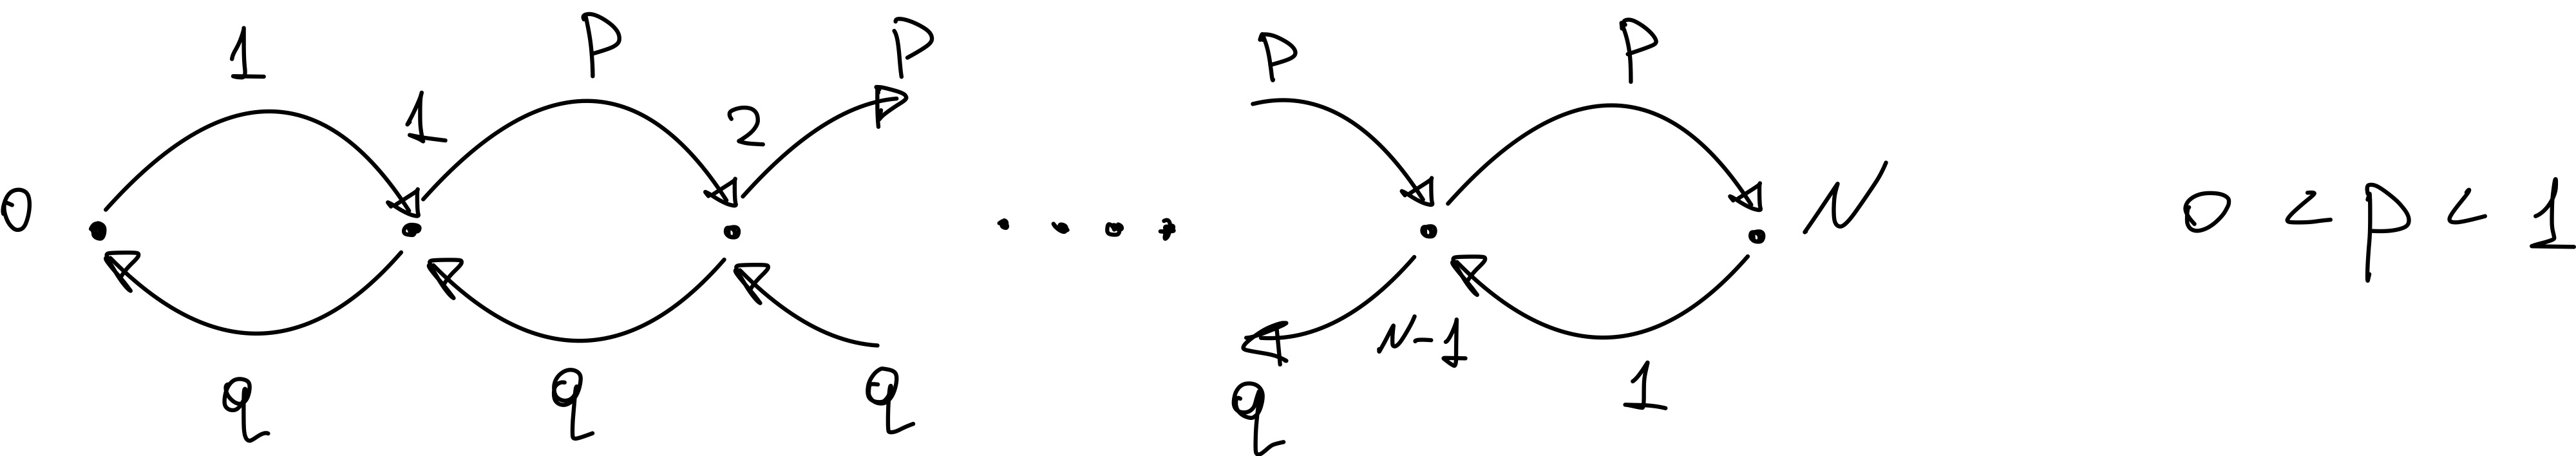
\includegraphics[width=0.8\textwidth]{fscanf_pic_bluzhdanie.JPG}
\end{figure}

Состояния цепи образуют здесь один неразложимый класс. Они  являются положительно возвратными с периодом $d = 2$. Из основной теоремы о стационарных распределениях (теорема \ref{th2}), у рассматриваемой цепи \textit{существует} и \textit{единственно} стационарное распределение $\mathbb{Q} = \{ q_0, q_1, ..., q_N \}$. Решая систему уравнений $q_j = \sum_{i = 0}^N q_i p_{ij}$ с условием $\sum_{i = 0}^N q_i = 1, \  q_i \geq 0, \  j \in E $, находим, что:
\begin{equation}\label{pi_i}
q_j = \frac{ \left( \frac{p}{q} \right)^{j - 1} }{1 + \sum_{j = 1}^{N - 1} \left( \frac{p}{q} \right)^{j - 1} }, \  2 \leq j \leq N - 1
\end{equation}
и $q_0 = q_1 q$, $q_N = q_{N - 1} p$.

Эргодическое распределение отсутствует -- это следует из основной теоремы об эргодических распределениях (теорема \ref{th3}) и того факта, что у рассматриваемой цепи период $d = 2$. Можно и непосредственно убедиться в том, что здесь нет эргодического распределения. Пусть, например, $N = 2$:
\begin{figure}[H]
    \centering
    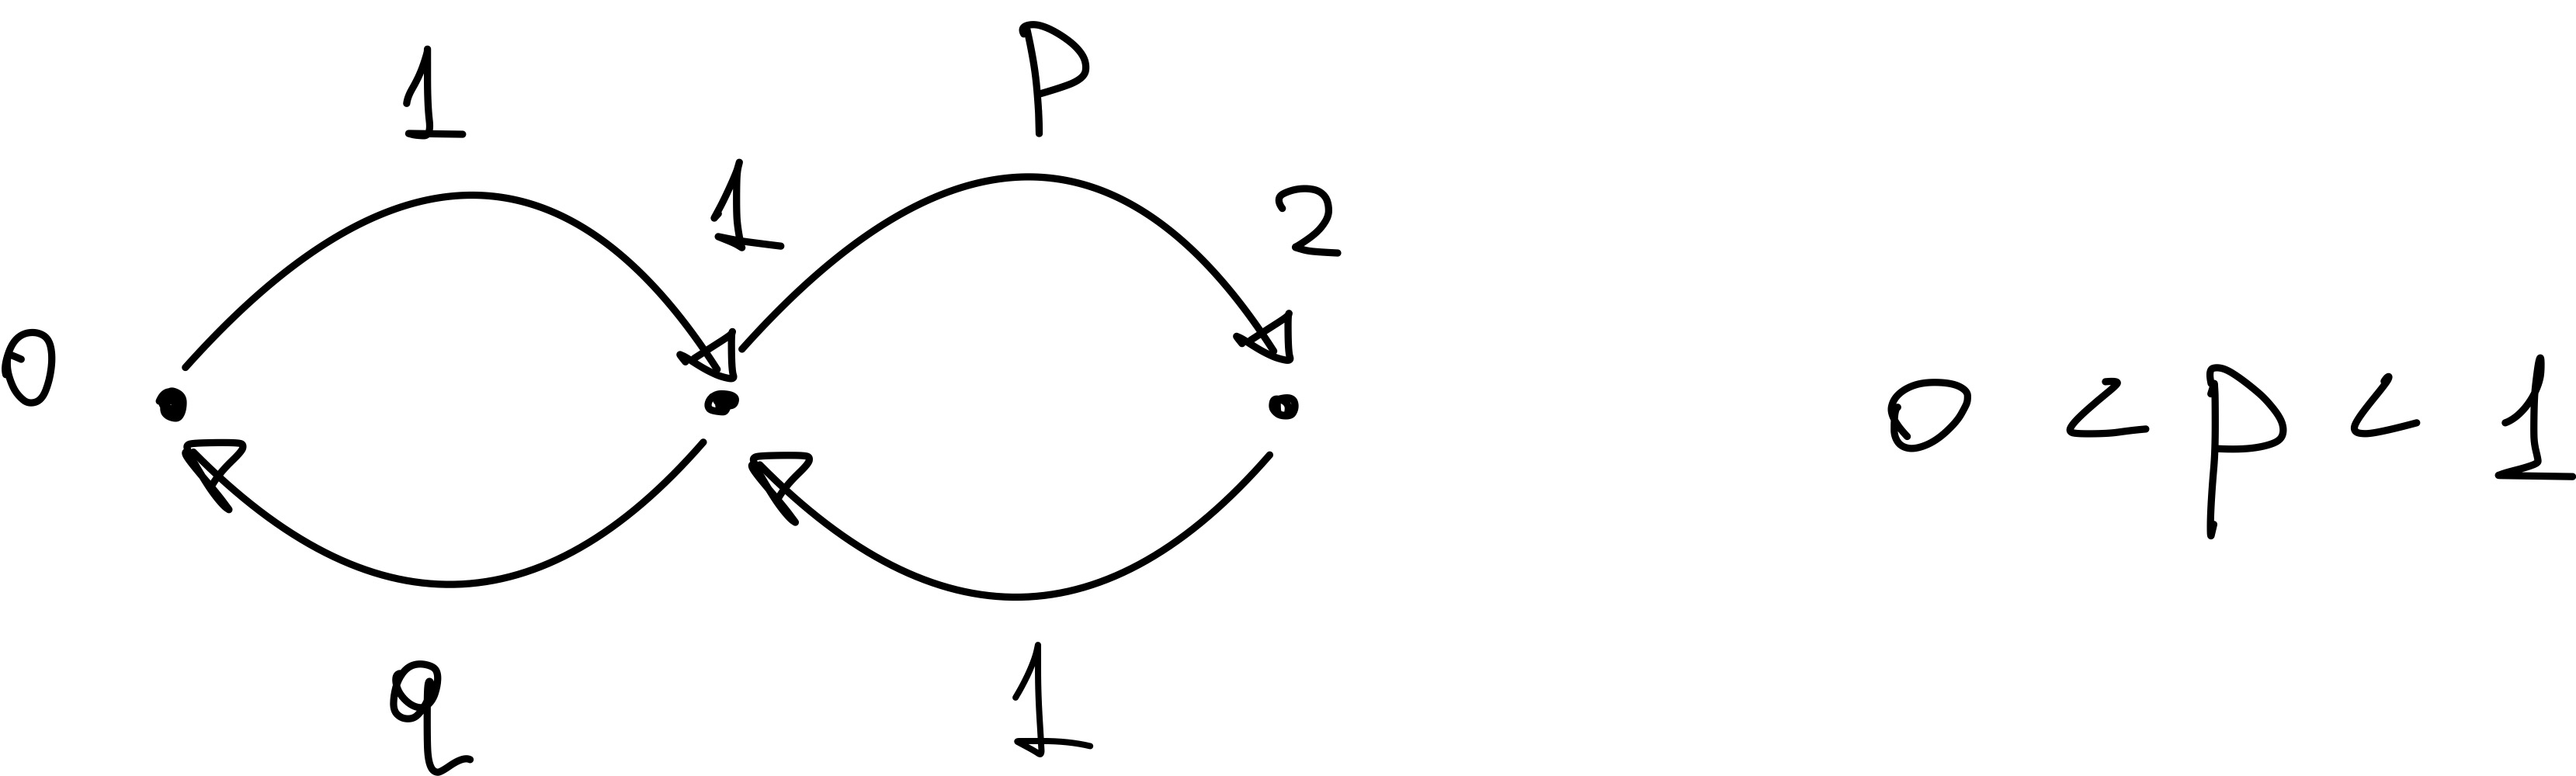
\includegraphics[width=0.5\textwidth]{fscanf_pic_bluzhdanie2.JPG}
\end{figure}

Тогда видно, что $p_{11}^{2n} = 1$, но $p_{11}^{2n + 1} = 0$. Так что $\lim_n p_{11}^{(n)}$ не существует. В то же самое время стационарное распределение \[ \mathbb{Q} = (q_0, q_1, q_2) \] есть, и, как следует из \eqref{pi_i}, оно имеет вид:
$$
q_0 = \frac{1}{2} q, \  q_1 = \frac{1}{2}, \  q_2 = \frac{1}{2} p
$$

\paragraph{Примеры применения}

Случайные блуждания на конечном множестве с отражающими экранами находят применение в различных областях, включая физику, экономику и теорию управления.

Один из примеров -- моделирование диффузии в физике. В этом случае цепь Маркова описывает движение частиц в системе, где отражающие экраны соответствуют границам реактора. Моделирование такого процесса позволяет оценить, как быстро распространяются частицы и как они взаимодействуют друг с другом.

В экономике случайные блуждания могут использоваться для моделирования цен на акции или валютные курсы. В этом случае цепь Маркова описывает изменение цен на основе предыдущих значений. Это позволяет анализировать поведение рынка и прогнозировать будущие цены.

В теории управления случайные блуждания используются для моделирования процессов принятия решений. Например, можно использовать цепь Маркова для моделирования процесса выбора определенной стратегии в зависимости от предыдущих решений. Это может помочь определить оптимальную стратегию и принять решение на основе вероятностных расчетов.

Таким образом, случайные блуждания на конечном множестве с отражающими экранами являются важным инструментом для моделирования случайных процессов в различных областях. Изучение свойств и теорем, связанных с цепями Маркова, позволяет более глубоко понимать эти процессы и использовать их для прогнозирования и принятия решений.

\paragraph{Заключение}

Случайные блуждания на конечном множестве с отражающими экранами -- это важный инструмент для моделирования случайных процессов в различных областях, таких как физика, экономика и теория управления. В физике они используются для моделирования диффузии частиц, а в экономике - для прогнозирования цен на акции или валютные курсы. В теории управления они помогают определить оптимальную стратегию и принять решение на основе вероятностных расчетов.

Изучение свойств и теорем, связанных с цепями Маркова, позволяет более глубоко понимать эти процессы и использовать их для прогнозирования и принятия решений. Важно отметить, что при моделировании случайных процессов необходимо учитывать все возможные факторы, которые могут повлиять на результаты. Также необходимо оценивать точность моделирования и корректировать ее при необходимости.

В целом, случайные блуждания на конечном множестве с отражающими экранами - это мощный инструмент для анализа случайных процессов. Их применение в различных областях позволяет получать более точные прогнозы и принимать более обоснованные решения.

